\long\def\comment#1{}

\subsection{Model}
\label{sec:methods:markov-setup}

We begin by detailing a parametric generative model for the (unobserved) joint spike trains of all $N$ observable neurons, along with the observed calcium fluorescence data. Each neuron is modeled as a generalized linear model (GLM). This class of models is known to capture the statistical firing properties of individual neurons fairly accurately \cite{BRIL88,CSK88,BRIL92,PG00,PILL07,PAN03d,PAN04c,Rigat06,TRUC05,NYK06,KP06,Vidne08,Stevenson2009}. We denote the $i$-th neuron's activity at time $t$ as $n_i(t)$: in continuous time, $n_i(t)$ could be modeled as an unmarked point process, but we will take a discrete-time approach here, with each $n_i(t)$ taken to be a binary random variable. We model the spiking probability of neuron $i$ via an instantaneous nonlinear function, $f(\cdot)$, of the filtered and summed input to that neuron at that time, $J_i(t)$. This input is composed of: (i) some baseline value, $b_i$; (ii) some external vector stimulus, $S^{ext}(t)$, that is linearly filtered by $k_i$; and (iii) spike history terms, $h_{ij}(t)$, encoding the influence on neuron $i$ from neuron $j$, weighted by $\w_{ij}$:
\begin{equation} \label{eqn:glm:definition}
\begin{array}{l}
n_i(t) \sim \text{Bernoulli}\left[f\left(J_i(t) \right) \right], \qquad
J_i(t)=b_i+k_i\cdot S^{ext}(t)+\sum \limits_{j=1}^{N} \w_{ij} h_{ij}(t).
\end{array}
\end{equation}

To ensure computational tractability of the parameters inference problem, we must impose some reasonable constraints on the instantaneous nonlinearity $f(\cdot)$ (which plays the role of the inverse of the link function in the standard GLM setting) and on the dynamics of the spike-history effects $h_{ij}(t)$. First, we restrict our attention to functions $f(\cdot)$ which ensure the concavity of the spiking loglikelihood in this model \cite{PAN04c,Escola07}, as we will discuss at more length below. In this paper, we use
\begin{equation}
f(J) = P\left[n>0 ~|~ n \sim \text{Poiss}\left(e^J\Delta\right)\right] = 1 - \exp[-e^J \Delta]
\end{equation}
(Fig.~\ref{fig:egfluor}), where the inclusion of $\Delta$, the time step size, ensures that the firing rate scales properly with respect to the time discretization; see \cite{Escola07} for a proof that this $f(\cdot)$ satisfies the required concavity constraints. However, we should note that in our experience the results depend only weakly on the details of $f(\cdot)$ within the class of log-concave models \cite{LD89,PAN04c}.

\begin{figure}[t!]
\centering 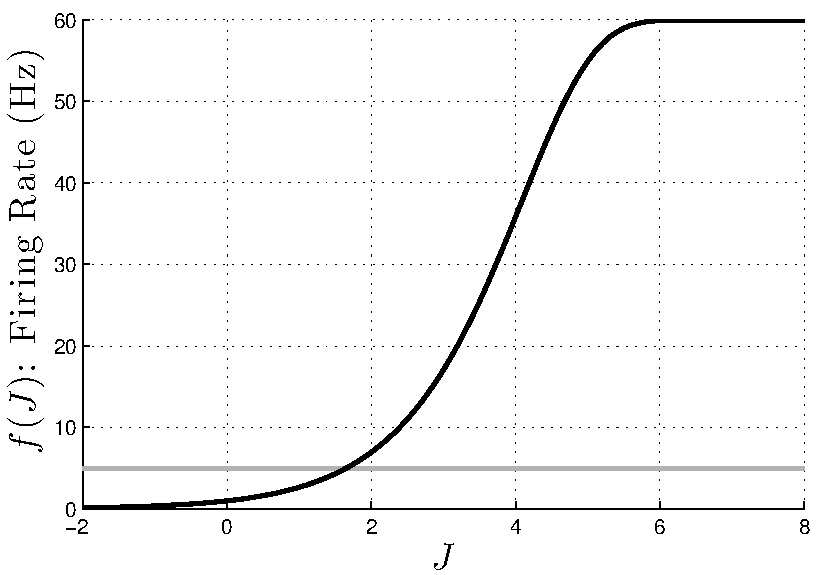
\includegraphics[width=3in]{../figs/fr_vs_J}
\caption{A plot of the firing rate nonlinearity $f(J)$ used in our
  simulations.  Note that the firing
  rate saturates at $1/\Delta$, because of our Bernoulli assumption
  (i.e., the spike count per bin is at most one). Here $\Delta = (60$
  Hz$)^{-1}$.}
\label{fig:egfluor}
\end{figure}

Second, because the algorithms we develop below assume Markovian dynamics, we model the spike history terms as an autoregressive process:
\begin{equation} \label{eqn:h:definition}
h_{ij}(t) = (1- \Delta/\tau^h_{ij}) h_{ij}(t- \Delta) +n_j(t) + \sigma^h_{ij}
  \sqrt{\Delta} \epsilon^h_{ij}(t),
\end{equation}
where $\tau^h_{ij}$ is the decay time constant for spike history terms, $\sigma^h_{ij}$ is a standard deviation parameter, $\sqrt{\Delta}$ ensures that the statistics of this Markov process have a proper Ornstein-Uhlenbeck limit as $\Delta \to 0$, and throughout this paper, $\epsilon$ denotes an independent standard normal random variable. Note that this model generalizes (via a simple augmentation of the state variable $h_{ij}(t)$) to allow each neuron to have several spike history terms, each with a unique time constant, which when weighted and summed allow us to model a wide variety of possible post-synaptic effects, including bursting, facilitating, and depressing synapses; see \cite{Vogelstein2009} for further details. We restrict our attention to the case of a single time constant $\tau^h_{ij}$ here, so the deterministic part of $h_{ij}(t)$ is a simple exponential function. Furthermore, we assume that $\tau^h_{ij}$ is the same for all neurons and all synapses, although in principle each synapse could be modeled with its unique $\tau^h_{ij}$. We do that both for simplicity and also because we find that the detailed shape of the coupling terms $h_{ij}(t)$ had a limited effect on the inference of the connectivity matrix, as illustrated in Fig.~\ref{fig:vartau} below. Thus, we treat $\tau^h_{ij}$ and $\sigma^h_{ij}$ as known synaptic parameters which are the same for each neuron pair $(i,j)$; therefore our unknown model spiking parameters are $\{\bw_i,k_i,b_i\}_{i\leq N}$, with $\bw_i=(\w_{i1},\ldots, \w_{iN})$.

The problem of estimating the connectivity parameters $\bw=\{\bw_i\}_{i\leq N}$ in this type of GLM, given a fully-observed ensemble of neural spike train $\{n_i(t)\}_{i\leq N}$, has recently received a great deal of attention; see the references above for a partial list. In the calcium fluorescent imaging setting, however, we do not directly observe spike trains; $\{n_i(t)\}_{i\leq N}$ must be considered a hidden variable here. Instead, each spike in a given neuron leads to a rapid increase in the intracellular calcium concentration, which then decays slowly due to various cellular buffering and extrusion mechanisms. We in turn make only noisy, indirect, and subsampled observations of this intracellular calcium concentration, via fluorescent imaging techniques \cite{ImagingManual}. To perform statistical inference in this setting, \cite{Vogelstein2009} proposed a simple conditional first-order hidden Markov model (HMM) for the intracellular calcium concentration $C_i(t)$ in cell $i$ at time $t$, along with the observed fluorescence, $F_i(t)$:
\begin{align}
\label{eqn:ca:definition}
C_i(t) &= C_i(t-\Delta) + (C_i^b-C_i(t-\Delta)) \Delta/\tau^c_i + A_i
n_i(t)+\sigma^c_i \sqrt{\Delta} \epsilon^c_i(t), \\ F_i(t) &= \alpha_i
S(C_i(t)) + \beta_i + \sqrt{\gamma_i S(C_i(t)) + \sigma^F_i}
\epsilon^F_i(t). \label{eqn:F:definition}
\end{align}
This model can be interpreted as a simple driven autoregressive process: under nonspiking conditions, $C_i(t)$ fluctuates around the baseline level of $C_i^b$, driven by normally-distributed noise $\epsilon^c_i(t)$ with standard deviation $\sigma^c_i \sqrt{\Delta}$. Whenever the neuron fires a spike, $n_i(t)=1$, the calcium variable $C_i(t)$ jumps by a fixed amount $A_i$, and subsequently decays with time constant $\tau^c_i$. The fluorescence signal $F_i(t)$ corresponds to the count of photons collected at the detector per neuron per imaging frame. This photon count may be modeled with normal statistics, with the mean given by a scaled and shifted Hill function $S(C)=C/(C+K_d)$ \cite{Yasuda2004} and the variance proportional to the mean (which follows from assuming the Poisson statistics of the photon counts are well approximated with Normal distribution; see \cite{Vogelstein2009} for further discussion. Because the parameter $K_d$ effectively acts as a simple scale factor, and is a property of the fluorescent indicator, we assume throughout this work that it is known. Figure \ref{fig:example_traces} shows a couple examples depicting the relationship between spike trains and observations.

\begin{figure}
\centering
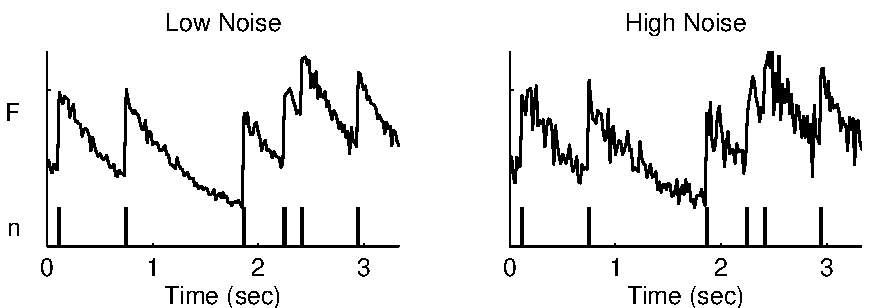
\includegraphics[width=\hsize]{../figs/sim_examples}
\caption{Both a low and high noise simulation showing typical relationships between spike trains and observations. Note that both panels have the same underlying spike train. Simulation parameters: $k_i=0.7$, $C_i^b=1$ $\mu$M, $\tau^c_i=500$ msec, $A_i=50$ $\mu$M, $\sigma^c_i=0.1$ $\mu$M,  $\alpha=2$, $\beta=0$, $\gamma=0.004, \, 0.016$ (left panel, right panel, respectively), $\sigma^F_i=0$.  $\Delta=1/60$ Hz.}
\label{fig:example_traces}
\end{figure}

To summarize, Eqs.~\eqref{eqn:glm:definition} -- \eqref{eqn:F:definition} define a coupled HMM: the underlying spike trains $\{n_i(t)\}_{i\leq N}$ and spike history terms $\{h_{ij}(t)\}_{i,j\leq N}$ evolve in a Markovian manner given the stimulus $S^{ext}(t)$. These spike trains in turn drive the intracellular calcium concentrations $\{C_i(t)\}_{i\leq N}$, which are themselves Markovian, but evolving at a slower timescale $\tau_i^c$. Finally, we observe only the fluorescence signals $\{F_i(t)\}_{i\leq N}$, which are related in a simple Markovian fashion to the calcium variables $\{C_i(t)\}_{i\leq N}$.

\subsection{Goal and general strategy}  \label{sec:methods:goal}

Our primary goal is to estimate the connectivity matrix, $\bw$, given the observed set of calcium fluorescence signals $\bF=\{\bF(t)\}_{t\leq T}$ and $\bF(t)=\{F_i(t)\}_{i\leq N}$. We must also deal with a number of nuisance parameters, $\tbth_i$: the intrinsic dynamics parameters $\{k_i, b_i, w_{ii}\}_{i\leq N}$, the calcium parameters $\{C^b_i, \tau^c_i, A_i, \sigma^c_i\}_{i\leq N}$, and the observation parameters $\{\alpha_i, \beta_i, \gamma_i, \sigma^F_i\}_{i\leq N}$. We addressed the problem of estimating these latter parameters in earlier work \cite{Vogelstein2009}; thus our focus here will be on the connectivity matrix $\bw$. A Bayesian approach is natural here, since we have a good deal of prior information about neural connectivity; see \cite{Rigat06} for a related discussion. However, a fully-Bayesian approach, in which we numerically integrate over the very high-dimensional parameters' space $\bth= \{\bth_i\}_{i\leq N}$, where $\bth_i=\{\bw_i, k_i, b_i, C^b_i, \tau^c_i, A_i, \sigma^c_i, \alpha_i, \beta_i, \gamma_i, \sigma^F_i\}$, is not particularly attractive from a computational point of view\footnote{The nuisance parameters for neuron $i$ are all its parameters, minus the cross-coupling terms, i.e.\ $\tbth_i =\bth_i \backslash \{w_{ij}\}_{i\neq j}$.}. Thus, our compromise is to compute \emph{maximum a posteriori} (MAP) estimates for the parameters via an expectation-maximization (EM) algorithm in which the sufficient statistics are computed by a hybrid blockwise Gibbs sampler and sequential Monte Carlo (SMC) method. More specifically, we iterate the steps:
\begin{align*}
\textbf{E step} &\text{: Evaluate } Q(\bth,\bth^{(l)}) = E_{P[\bX |
\bF; \bth^{(l)}]} \ln P \left[ \bF, \bX | \bth \right] = \int P[\bX |
\bF; \bth^{(l)}] \ln P[\bF, \bX | \bth] d \bX \\ \textbf{M step}
&\text{: Solve } \bth^{(l+1)} = \argmax_{\bth} \left\{
Q(\bth,\bth^{(l)}) + \ln P(\bth) \right\},
\end{align*}
where $\bX$ denotes the set of all hidden variables $\{ C_i(t), n_i(t), h_{ij}(t) \}_{i,j \leq N, t \leq T}$ and $P(\bth)$ denotes a (possibly improper) prior on the parameter space $\bth$. According to standard EM theory \cite{DLR77,McLachlanKrishnan96}, each iteration of these two steps is guaranteed to increase the log-posterior $\ln P(\bth^{(l)} | \bF)$, and will therefore lead to at least a locally maximum a posteriori estimator.

Now, our major challenge is to evaluate the auxiliary function $Q(\bth,\bth^{(l)})$ in the E-step. Our model is a coupled HMM, as discussed in the previous section; therefore, as usual in the HMM setting \cite{RAB89}, $Q$ may be broken up into a sum of simpler terms: 
\begin{eqnarray} 
Q(\bth,\bth^{(l)}) 
&=& \sum_{it} P[C_i(t) | F_i; \tbth_i] \times \ln P[F_i(t)|C_i(t); \alpha_i, \beta_i, \gamma_i, \sigma^F_i] \nonumber \\ 
&+& \sum_{it} P[C_i(t), C_i(t-\Delta), n_i(t) | F_i; \tbth_i] \times \ln P[C_i(t)|C_i(t-\Delta), n_i(t); C^b_i, \tau^c_i, A_i, \sigma^c_i] \nonumber \\ 
&+& \sum_{it} P[n_i(t), \bh_i(t) | \bF; \bth_i] \times \ln P[n_i(t)| \bh_i(t); b_i, k_i, \bw_i, S^{ext}(t)] 
% \nonumber \\
% &+& \sum_{it} P[h_i(t), h_i(t-\Delta),n_i(t) | F_i; \tbth_i] \times \ln P[h_i(t)| h_i(t-\Delta), n_i(t); \tau^h, \sigma^h], 
\label{eqn:loglik:definition-expl} 
\end{eqnarray} 
\noindent where $\bh_i(t)=\{h_{ij}(t)\}_{j \leq N}$. Note that each of the three sums here corresponds to a different component of the model described in Eqs.~\eqref{eqn:glm:definition} -- \eqref{eqn:F:definition}: the first sum involves the fluorescent observation parameters, the second the calcium dynamics, and the third the spiking dynamics (note the absence of a term for the spike history terms, as their parameters are assumed known a priori).

Thus we need only compute low-dimensional marginals of the full posterior distribution $P[\bX | \bF; \bth]$; specifically, we need pairwise marginals, of the form $P[C_i(t), C_i(t- \Delta) | F_i; \tbth_i]$, and marginals $P[C_i(t)|F_i;\tbth_i]$ and $P[n_i(t),\bh_i(t)|\bF;\bth_i]$. Details for calculating $P[C_i(t), C_i(t- \Delta) | F_i; \tbth_i]$ and $P[C_i(t)|F_i;\tbth_i]$ are found in \cite{Vogelstein2009}. Calculation of the joint marginal for high dimensional hidden variable $\bh_i$ necessitates the development of specialized blockwise Gibbs-SMC sampling method, as we describe in the subsequent sections \ref{sec:methods:indep} and \ref{sec:methods:joint}. Once we have obtained these marginals, the M-step breaks up into a number of independent optimizations that may be computed in parallel and which are therefore relatively straightforward (Section \ref{sec:methods:parameters HMM}); see section \ref{sec:methods:specific_implementation} for a pseudocode summary along with some specific implementation details.

\subsection{Initialization of nuisance parameters via sequential
  Monte Carlo methods} \label{sec:methods:indep}

We begin by constructing relatively cheap, approximate preliminary estimators for the nuisance parameters, $\tbth_i$.
%= \bth \backslash \{w_{ij}\}_{i\neq j}$, i.e., the observation parameters, $\{\alpha_i,\beta_i,\gamma_i,\sigma^F_i\}$, the calcium dynamics parameters $\{C^b_i,\tau^c_i, A_i, \sigma^c_i\}_i$, and the intrinsic spiking parameters, $\{k_i,b_i,w_{ii}\}$.
The idea is to initialize our estimator by assuming that each neuron is observed independently. Thus we want to compute $P[C_i(t), C_i(t-\Delta) | F_i; \tbth_i]$ and $P[C_i(t)|F_i;\tbth_i]$, and solve the M-step for each $\tbth_i$, with the connectivity matrix parameters held fixed. This single-neuron case is much simpler, and has been discussed at length in \cite{Vogelstein2009}; therefore, we only provide a brief overview here. The standard forward and backward recursions provide these posteriors \cite{ShumwayStoffer06}:
\begin{align}
% \hspace{-25mm}  
P[X_i(t) | F_i(0:t)] &\propto P[F_i(t)| X_i(t)] \int P[X_i(t) |
    X_i(t-\Delta)] P[X_i(t-\Delta) | F_i(0:t-\Delta)] dX_i(t-\Delta),
\label{eqn:forward} \\
% \hspace{-25mm} 
P[X_i(t), X_i(t-\Delta) | F_i] &= P[X_i(t) | F_i]
\frac{P[X_i(t) | X_i(t-\Delta)] P[X_i(t-\Delta) |
F_i(0:t-\Delta)]}{\int P[X_i(t) | X_i(t-\Delta)] P[X_i(t-\Delta) |
F_i(0:t-\Delta)] dX_i(t-\Delta)},
\label{eqn:backward}
\end{align}
where $F_i(s:t)$ denotes the time series $F_i$ from time points $s$ to $t$, and we have dropped the conditioning on the parameters for brevity's sake. Eq.~\eqref{eqn:forward} describes the forward (filter) pass of the recursion, and Eq.~\eqref{eqn:backward} describes the backward (smoother) pass, providing both $P[X_i(t), X_i(t-\Delta) | F_i]$ and $P[X_i(t)|F_i]$ (obtained by marginalizing by $X_i(t-\Delta)$).

Because these integrals cannot be analytically evaluated for our model, we approximate them using a SMC (``marginal particle filtering'') method \cite{DGA00,DFG01,GDW04}; see \cite{Vogelstein2009} for details on the proposal density and resampling methods used here. The output of this SMC method comprises an array of particle positions $\{X_i^{(m)}(t)\}_{m=1}^{M}$, where $m$ indexes the particle number, and a discrete approximation to the marginals $P[X_i(t), X_i(t-\Delta) | F_i]$,
\begin{multline}
% \begin{array}{rl}
P[X_i(t), X_i(t-\Delta) | F_i] \approx \\
\approx \sum_{m,m'}
r_i^{(m,m')}(t,t-\Delta) \delta \left[ X_i(t) - X_i^{(m)}(t) \right]
\delta \left[ X_i(t-\Delta) - X_i^{(m')}(t-\Delta) \right],
% \end{array}
\label{eqn:particle-fb}
\end{multline}
where $r_i^{(m,m')}(t,t-\Delta)$ denotes the weight attached to the
pair of particles with positions $\left( X_i^{(m)}(t),
X_i^{(m')}(t-\Delta) \right)$, and $\delta(.)$ denotes a Dirac mass.

As discussed above, the sufficient statistics for estimating the nuisance parameters for each neuron, $\tbth_i$, are exactly these marginal posteriors. As discussed following Eq.~\eqref{eqn:loglik:definition-expl}, the M-step decouples into three independent subproblems. The first term depends on only $\{\alpha_i, \beta_i, \gamma_i, \sigma_i\}$; since $P[F_i(t)|S(C_i(t)); \tbth_i]$ is quadratic (by our Gaussian assumption on the fluorescent observation noise), we can estimate these parameters by solving a weighted regression problem (specifically, we use a coordinate-optimization approach: we solve a quadratic problem for $\{\alpha_i, \beta_i\}$ while holding $\{\gamma_i, \sigma_i\}$ fixed, then estimate $\{\gamma_i,\sigma_i\}$ by the usual residual error formulas while holding $\{\alpha_i, \beta_i\}$ fixed). Similarly, the second term requires us to optimize over $\{\tau_i^c, A_i, C_i^b\}$, and then we use the residuals to estimate $\sigma_i^c$. Note that all the parameters mentioned so far are constrained to be non-negative, but may be solved efficiently using standard quadratic program solvers if we use the simple reparameterization $\tau_i^c \to 1- \Delta / \tau_i^c$. Finally, the last term, assuming neurons are independent, may be expanded:
\begin{multline}
E [\ln P[n_i(t), \bh_i(t) | \bF; \bth_i]] =  \\ = P[n_i(t), \bh_i(t) |
\bF] \ln f [J_i(t)] + (1-P[n_i(t), \bh_i(t) | \bF]) \ln [1-
f(J_i(t))];
\label{eqn:bw}
\end{multline}
since $J_i(t)$ is a linear function of $\{b_i,k_i,\bw_i\}$, and the right-hand side of Eq.~\eqref{eqn:bw} is concave in $J_i(t)$, we see that the third term in Eq.~\eqref{eqn:loglik:definition-expl} is a sum of terms which are concave in $\{b_i,k_i,\bw_i\}$ --- and therefore also concave in the linear subspace $\{b_i,k_i, w_{ii}\}$ with $\{w_{ij}\}_{i \neq j}$ held fixed --- and may thus be maximized efficiently using any convex optimization method, e.g.\ Newton-Raphson or conjugate gradient ascent.

Our procedure therefore is to initialize the parameters for each neuron using some default values that we have found to be practically effective in analyzing real data, and then recursively (i) estimate the marginal posteriors via Eq.~\eqref{eqn:particle-fb} (E step), and (ii) maximize the nuisance parameters $\tbth_i$ (M step), using the above described approach. We iterate these two steps until the change in $\tbth_i$ does not exceed some minimum threshold (or we reach an upper bound on iterations). We then use the marginal posteriors from the last iteration to seed the blockwise Gibbs sampling procedure described below. With that, we approximate $P[n_i,\bh_i | \bF;\bth_i]$.

\subsection{Estimating joint posteriors over weakly coupled neurons}
\label{sec:methods:joint}

Now we turn to the key problem: constructing an estimate of the joint marginals $\{P[n_i(t), \bh_i(t) | \bF;\bth]\}_{i\leq N}$, which are the sufficient statistics for estimating the connectivity matrix $\bw$ (recall Eq.~\eqref{eqn:loglik:definition-expl}). The SMC method described in the preceding section only provide the marginals over each neuron; this method may in principle be extended to obtain the desired full posterior $P[\bX(t), \bX(t-\Delta) | \bF; \bth]$, but the SMC is fundamentally a sequential importance sampling method, and therefore scales poorly as the dimensionality of the hidden state $\bX(t)$ increases \cite{BickelBengtsson08}. Thus we need a different approach.

One very simple idea is to use a Gibbs sampler: sample sequentially
from
\begin{align}
X_i(t) \sim P[X_i(t) | \bX_{\i}, X_i(0), \ldots, X_i(t-\Delta),
 X_i(t+\Delta), \ldots, X_i(T), \bF; \bth],
\end{align}
looping over all cells $i$ and all time bins $t$. Unfortunately, this approach is likely to mix poorly, due to the strong temporal dependence between $X_i(t)$ and $X_i(t+\Delta)$. Instead, we propose a blockwise Gibbs strategy, sampling one spike train as a block:
\begin{align}
	X_i \sim P[X_i | \bX_{\i}, \bF; \bth].
\end{align}
If we can draw these blockwise samples $X_i = X_i(s:t)$ efficiently for a large subset of $t-s$ adjacent time-bins simultaneously, then we would expect the resulting Markov chain to mix much more quickly than the single-element Gibbs chain.  This follows due to the weak dependence between $X_i$ and $X_j$ when $i\neq j$, and that Gibbs is most efficient for weakly-dependent variables \cite{RC05}.

So, how can we efficiently sample from $P[X_i | \bX_{\i}, \bF; \bth]$? One attractive approach is to try to re-purpose the SMC method described above, which is quite effective for drawing approximate samples from $P[X_i | \bX_{\i}, F_i; \bth]$ for one neuron $i$ at a time. Recall that sampling from an HMM is in principle easy by the ``propagate forward, sample backward'' method: we first compute the forward probabilities $P[X_i(t) | \bX_{\i}(0:t), F_i(0:t); \bth]$ recursively for timesteps $0$ up to $T$, then sample backwards from $P[X_i(t) | \bX_{\i}(0:T), F_i(0:T), X_i(t-\Delta); \bth]$. This approach is powerful because each sample requires just linear time to compute (i.e., $O(T/\Delta)$ time, where $T/\Delta$ is the number of desired time steps). Unfortunately, in this case we can only compute the forward probabilities approximately (with the SMC forward recursion approximation to Eq.~\eqref{eqn:forward}), and so therefore this attractive forward-backward approach only provides approximate samples from $P[X_i | \bX_{\i}, \bF; \bth]$, not the exact samples required for the validity of the Gibbs method.

Of course, in principle we should be able to use the Metropolis-Hastings (M-H) algorithm to correct these approximate samples. The problem is that the M-H acceptance ratio in this setting involves a high-dimensional integral over the set of paths that the particle filter might possibly trace out, and is therefore difficult to compute directly. \cite{Andrieu2007} discuss this problem at more length, along with some proposed solutions. A slightly simpler approach was introduced by \cite{NBR03}. Their idea is to exploit the $O(T/\Delta)$ forward-backward sampling method by embedding a discrete Markov chain within the continuous state space $\mathcal{X}_t$; the state space of this discrete embedded chain is sampled randomly according to some distribution $\rho_t$ with support on $\mathcal{X}_t$. It turns out that an appropriate acceptance probability (defined in terms of the original state space model transition and observation probabilities, along with the auxiliary sampling distributions $\rho_t$) may be computed quite tractably, guaranteeing that the samples produced by this algorithm form a Markov chain with the desired equilibrium density. See \cite{NBR03} for details.

We can apply this embedded-chain method quite directly here to sample from $P[X_i | \bX_{\i}, \bF; \bth]$. The one remaining question is how to choose the auxiliary densities $\rho_t$. We would like to choose these densities to be close to the desired marginal densities $P[X_i(t) | \bX_{\i}, \bF; \bth]$, and conveniently, we have already computed a good (discrete) approximation to these densities, using the SMC methods described in the last section. The algorithm described in \cite{NBR03} requires that $\rho_t$ be continuous densities, so we simply convolve our discrete SMC-based approximation (specifically, the $X_i(t)$-marginal of Eq.~\eqref{eqn:particle-fb}) with an appropriate normal density to arrive at a very tractable mixture-of-Gaussians representation for $\rho_t$ with required properties.

Thus, to summarize, our procedure for approximating the desired joint state distributions $P[n_i(t), \bh_i(t) | \bF;\bth_i]$ has a Metropolis-within-blockwise-Gibbs flavor, where the internal Metropolis step is replaced by the $O(T/\Delta)$ embedded-chain method introduced by \cite{NBR03}, and the auxiliary densities $\rho_t$ necessary for implementing the embedded-chain sampler are obtained using the SMC methods from \cite{Vogelstein2009}.

\subsubsection{A factorized approximation of the joint posteriors}
\label{sec:cheaper-high-snr}

If the SNR in the calcium imaging is sufficiently high, then by definition the observed fluorescence data $F_i$ will provide enough information to determine the underlying hidden variables $X_i$. Thus, in this case the joint posterior approximately factorizes into a product of marginals for each neuron $i$:
\begin{equation} \label{eqn:indep_approx}
  P[\bX(t)|\bF;\bth] \approx \prod_{i\leq N} P[X_i(t)|F_i;\tbth_i].
\end{equation}
We can take advantage of this because we have already estimated all the above marginals using the SMC method in Section \ref{sec:methods:indep}. %In particular, we can obtain the sufficient statistics $P[n_i(t), \bh_i(t) | \bF;\tbth_i]$ by forming a product over the marginals $P[X_i(t) | F_i,\tbth_i]$ obtained from Eq.~\eqref{eqn:particle-fb}. 
This factorized approximation entails a very significant gain in efficiency for two reasons: first, it obviates the need to generate joint samples via the expensive blockwise-Gibbs approach described above; and second, because we can very easily parallelize the SMC step, inferring the marginals $P[X_i(t) | F_i; \tbth_i]$ and estimating the parameters $\bth_i$ for each neuron on a separate processor. We will discuss the empirical accuracy of this approximation the Results section.

\subsection{Estimating the functional connectivity matrix} \label{sec:methods:parameters HMM}

Computing the M-step for the connectivity matrix, $\bw$, is an optimization problem with on the order of $N^2$ variables. The auxiliary function Eq.~\eqref{eqn:loglik:definition-expl} is concave in $\bw$, and decomposes into $N$ separable terms that may be optimized independently using standard ascent methods. To improve our estimates, we will incorporate two sources of strong \emph{a priori} information via our prior $P(\bw)$: first, previous anatomical studies have established that connectivity in many neuroanatomical substrates is ``sparse,'' i.e., most neurons form synapses with only a fraction of their neighbors \cite{Buhl94,Thompson88,Reyes98,Feldmeyer99,Gupta00,FeldmeyerSakmann00,PetersenSakmann00,Binzegger04,Song2005,Mishchenko2009b}, implying that many elements of the connectivity matrix $\bw$ are zero; see also \cite{PAN04c,Rigat06,PILL07,Stevenson08} for further discussion. Second, ``Dale's law'' states that each of a neuron's postsynaptic connections in adult cortex (and many other brain areas) must all be of the same sign (either excitatory or inhibitory). Both of these priors are easy to incorporate in the M-step optimization, as we discuss below.


\subsubsection{Imposing a sparse prior on the functional connectivity}

It is well-known that imposing sparseness via an $L1$-regularizer can dramatically reduce the amount of data necessary to accurately reconstruct sparse high-dimensional parameters \cite{Tibs96,TIP01,DE03,NG04,Candes2005,Mishchenko2009}. We incorporate a prior of the form $\ln p(\bw) = const. - \lambda \sum_{i,j} |\w_{ij}|$, and additionally enforce the constraints $|\w_{ij}|<M$, for a suitable constant $M$ (since both excitatory and inhibitory cortical connections are known to be bounded in size). Since the penalty $\ln p(\bw)$ is concave, and the constraints $|\w_{ij}|<M$ are convex, we may solve the resulting optimization problem in the M-step using standard convex optimization methods \cite{CONV04}. In addition, the problem retains its separable structure: the full optimization may be broken up into $N$ smaller problems that may be solved independently.

\subsubsection{Imposing Dale's law on the functional connectivity}

Enforcing Dale's law requires us to solve a non-convex, non-separable problem: we need to optimize the concave function $Q(\bth,\bth^{(l)}) + \ln P(\bth)$ under the non-convex, non-separable constraint that all of the elements in any column of the matrix $\bw$ are of a definite sign (either nonpositive or nonnegative). It is difficult to solve this nonconvex problem exactly, but we have found that simple greedy methods are quite efficient in finding good approximate solutions.

We begin with our original sparse solution, obtained as discussed in the previous subsection without enforcing Dale's law. Then we assign each neuron as either excitatory or inhibitory, based on the weights we have inferred in the previous step: i.e., neurons $i$ whose inferred postsynaptic connections $w_{ij}$ are largely positive are tentatively labeled excitatory, and neurons with largely inhibitory inferred postsynapic connections are labeled inhibitory. Neurons which are highly ambiguous may be unassigned in the early iterations, to avoid making mistakes from which it might be difficult to recover. Given the assignments $a_i$ ($a_i =1$ for putative excitatory cells, $-1$ for inhibitory, and $0$ for neurons which have not yet been assigned) we solve the convex, separable problem \begin{equation} \argmax_{\substack{a_i \w_{ij} \geq 0, |w_{ij}|<M ~ \forall i,j}} Q(\bth,\bth^{(l)}) - \lambda \sum_{ij} |w_{ij}| \end{equation} which may be handled using the standard convex methods discussed above. Given the new estimated connectivities $\bw$, we can re-assign the labels $a_i$, or even flip some randomly to check for local optima. We have found this simple approach to be effective in practice.


\subsection{Specific implementation notes} \label{sec:methods:specific_implementation}

Pseudocode summarizing our approach is given in Algorithm \ref{eqn:pseudocode}. As discussed in Section \ref{sec:methods:indep}, the nuisance parameters $\tbth_i$ may be initialized effectively using the methods described in \cite{Vogelstein2009}; then the full parameter $\bth$ is estimated via EM, where we use the embedded-chain-within-blockwise-Gibbs approach discussed in Section \ref{sec:methods:joint} (or the cheaper factorized approximation described in Section \ref{sec:cheaper-high-snr}) to obtain the sufficient statistics in the E step and the separable convex optimization methods discussed in Section \ref{sec:methods:parameters HMM} for the M step.

\begin{algorithm}[t!]
\caption{Pseudocode for estimating functional connectivity from
calcium imaging data using EM; $\eta_1$ and $\eta_2$ are
user-defined convergence tolerance parameters.}
\label{eqn:pseudocode}
\begin{algorithmic}
\While{$|{\bw}^{(l)}-{\bw}^{(l-1)}|>\eta_1$}
  \ForAll{$i=1\ldots N$}
    \While{$|{\tbth_i}^{(l)}-{\tbth_i}^{(l-1)}|> \eta_2$}
      \State Approximate $P[X_i(t)|F_i; \tbth_i]$ using SMC (Section \ref{sec:methods:indep})
      \State Perform the M-step for the nuisance parameters $\tbth_i$ (Section \ref{sec:methods:indep})
    \EndWhile
  \EndFor
      \ForAll{$i=1\ldots N$}
      \State Approximate $P[n_i(t), \bh_i(t) |\bF; \bth_i]$ using either the blockwise Gibbs
      \State method or the factorized approximation (Section \ref{sec:methods:joint})
    \EndFor
  \ForAll{$i=1\ldots N$}
  	\State Perform the M-step on $\bth_i$ using separable convex optimization methods (Section \ref{sec:methods:parameters HMM})
  \EndFor
\EndWhile
\end{algorithmic}
\end{algorithm}

As emphasized above, the parallel nature of these EM steps is essential for making these computations tractable. We performed the bulk of our analysis on a 100-node cluster of Intel Xeon L5430 based computers (2.66 GHz). For 10 minutes of simulated fluorescence data, imaged at $30$ Hz, calculations using the factorized approximation typically took 10-20 minutes per neuron (divided by the number of available processing nodes on the cluster), with time split approximately equally between (i) estimating the nuisance parameters $\tbth_i $, (ii) approximating the posteriors using the independent SMC method, and (iii) estimating the functional connectivity matrix, $\bw$. The hybrid embedded-chain-within-blockwise-Gibbs sampler was substantially slower, up to an hour per neuron per Gibbs pass, with the Gibbs sampler dominating the computation time, because we thinned the chain by a factor of five (since we found empirically that the autocorrelation of the Gibbs chain had a scale of about five time steps).

\begin{figure}[t!] 
	\centering 
	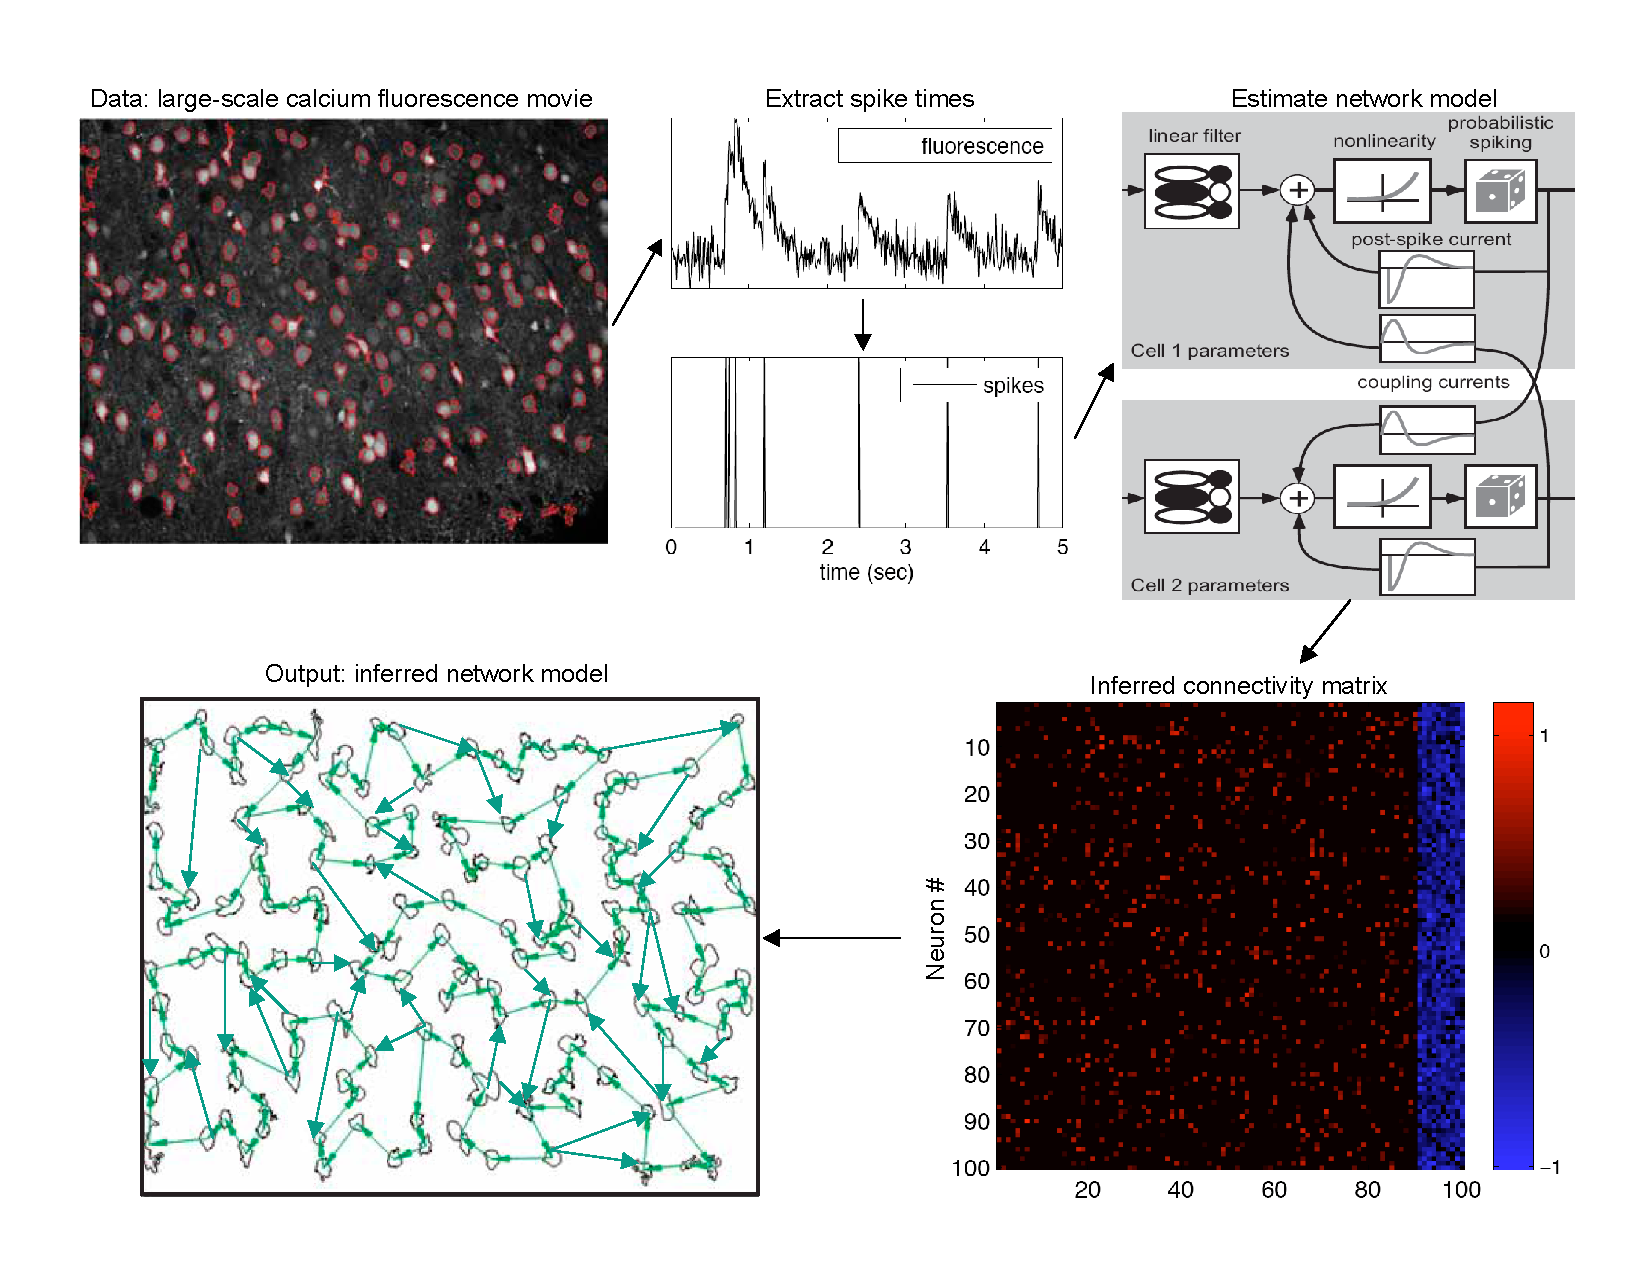
\includegraphics[width=\hsize]{../figs/yuri-paper-schematic} 
	\caption{Schematic overview. The raw observed data is a large-scale calcium fluorescence movie, which is pre-processed to correct for movement artifacts (in the in vivo setting) and find regions-of-interest (i.e., putative neurons); note that we have omitted details of these important preprocessing steps in this paper. Given the fluorescence traces from each neuron, we estimate the underlying spike trains (i.e., in time series of neural activity) using statistical deconvolution methods. Then we estimate the parameters of a network model, given the observed data. Our major goal is to obtain an accurate estimate of the network connectivity matrix, which summarizes the information we are able to infer about the local neuronal microcircuit. This figure adapted from personal communications with R.\ Yuste, B.\ Watson, and A.\ Packer.} 
	\label{fig:data_schematic} 
\end{figure}

\subsection{Simulating a neural population} \label{sec:results:simulations}

To test the described method for inferring functional connectivity from calcium imaging data, we simulated networks (according to our model, Eqs.~\eqref{eqn:glm:definition} -- \eqref{eqn:F:definition}) of spontaneously firing randomly connected neurons. Although simulations ran at $1$ msec time discretization, imaging rate was assumed to be much slower: $5$--$200$ Hz. Simulations lasted anywhere between 5 minutes and 1 hours (of simulated time). 

Model parameters were chosen based on experimental data available in the literature for cortical neural networks \cite{Braitenberg1998,Urquijo2000,Lefort2009,Sayer1990}. More specifically, the network contained 80\% of excitatory and 20\% inhibitory neurons \cite{Braitenberg1998,Urquijo2000}, each respecting Dale's law. Neurons were randomly connected to each other with probability $0.1$ \cite{Braitenberg1998,Lefort2009}. Synaptic weights for excitatory connections, as defined by EPSP peak amplitude, were randomly drawn from exponential distribution with the mean of $0.5 \mu V$ \cite{Lefort2009,Sayer1990}. Inhibitory connections were also drawn from exponential distribution; their strengths chosen so as to balance excitatory and inhibitory currents in the network, and achieve an average firing rate of $\approx 5 $ Hz \cite{Abeles91}. Practically, this meant that the mean strength of inhibitory connections was about 10 times larger than that of the excitatory connections. PSP shapes were modeled as an alpha function \cite{Koch99}, by differencing two exponentials, corresponding to a sharp rise and relatively slow decay \cite{Sayer1990}. We neglected conduction delays, given that the time delay below $\sim 1$ msec expected in local cortical circuit was smaller than the time step of our computer simulation. Each neuron also had an exponential refractory current \cite{Koch99}.

Note that EPSP peak amplitudes cannot be used directly in Eq.~\eqref{eqn:glm:definition}, as a synaptic weight in our model --- $w_{ij}$ in Eq.~\eqref{eqn:glm:definition} --- is a dimensionless quantity representing the change in the spiking probability of neuron $i$ given neuron $j$ fired; whereas EPSP peak amplitude describes physiologically measured change in the membrane voltage of a neuron due to synaptic currents triggered by spike in neuron $j$. We must therefore find a way to relate the two.

Consider the above model for spiking, Eqs.~\eqref{eqn:glm:definition} -- \eqref{eqn:h:definition}.  Let $\delta P$ be the difference between the probability of neuron $i$ spiking given that neuron $j$ spiked in the previous time bin, $P[n_i(t)=1 | n_j(t-\Delta)=1]$, and the probability of neuron $i$ spiking given that neuron $j$ did \emph{not} spike in the previous time bin, $P[n_i(t) | n_j(t-\Delta)=0]$:
\begin{align}\label{eqn:convert:leadin-2}
\delta P &= P[n_i(t)=1 | n_j(t-\Delta)=1] - P[n_i(t)=1 | n_j(t-\Delta)=0] \nonumber
\\ &= \exp[-e^{b_i+w_{ij}\tau_w}\Delta]-\exp[-e^{b_i}\Delta]
\end{align}
\noindent where $\tau_w$ accounts for the decay time constant of the spike history term.   Now consider a simple, stochastic, integrate-and-fire neuron, with baseline voltage zero, spiking threshold one, EPSP amplitude $V_E$, and variance $\sigma_v^2$:
\begin{align}
	V_i(t) &= V_i(t-\Delta) + V_E \delta(n_j(t-\Delta)) + \sigma_v \sqrt{\Delta} \varepsilon_i(t), \qquad &\text{if } V_i(t)<1 \nonumber
\\	V_i(t) &= 0 &\text{if } V_i(t)\geq 1 
\end{align}
In such a model, we again write $\delta P$:
\begin{align}\label{eqn:convert:leadin-3}
\delta P &= \int_1^\infty \mathcal{N}(V_i(t-\Delta),\sigma^2) \text{d}V_i(t-\Delta) - \int_1^\infty \mathcal{N}(V_i(t-\Delta)+V_E,\sigma^2)\text{d}V_i(t-\Delta) \nonumber
\\ &=g(V_E)
\end{align}
A little algebra yields:
\begin{align}
	w_{ij}= \frac{1}{\tau_w}\left(\ln \left[ -\frac{1}{\Delta} \ln \left[g(V_E)+ \exp\left(-\text{e}^{b_i}\Delta\right)\right]\right]-b_i\right)
\end{align}
which we used to obtain $\bw$ from the above mentioned parameters. 
% So, writing $w_{ij}$ as a function of our integrate and fire model, and plugging it back into Eq.~\eqref{eqn:glm:definition}, we say:
% \begin{equation}\label{eqn:convert}
% \w_{ij}\approx\ln(-\ln(e^{-r_i\tau^h}-V_E/V_b)/r_i\tau^h).
% \end{equation}
% \noindent where $r_i=\exp(b_i)$ is the base firing rate of neuron $i$. 


Parameters for the internal calcium dynamics and fluorescence observations were chosen according to our experience with several cells analyzed using algorithm of \cite{Vogelstein2009}, and conformed to previously published results \cite{ImagingManual,HelmchenSakmann96,BrenowitzRegehr07}. %Each parameter was generated from a normal distribution with specified mean and variance at about 30\% of the mean, truncated at the lower bound at about 30\% of the mean value.  
Table \ref{table:caparm} summarizes the details for each of the parameters in our model.

\begin{table}[h!b!p!]
\caption{Table of simulation parameters. $\mathcal{E}(\lambda)$ indicates an exponential distribution with mean $\lambda$, and $\mathcal{N}_p(\mu,\sigma^2)$ indicates a normal distribution with mean $\mu$ and variance $\sigma^2$, truncated at lower bound $p\mu$.  Units (when applicable) are given with respect to mean values (i.e., units are squared for variance).}\label{table:caparm}

\begin{tabular}{lll}
\hline
Total neurons & 10-500 & \# \\
Excitatory neurons & $80$ & $\%$ \\
Connections sparseness & $10$   & $\%$ \\
Baseline firing rate & $5$ & Hz\\
\hline
EPSP peak height 	& $\sim \mathcal{E}(0.5)$ & $\mu$V \\
IPSP peak height 	& $\sim -\mathcal{E}(2.3)$ & $\mu$V \\
EPSP rise time 		& 1 & msec \\
IPSP rise time 		& 1 & msec \\
EPSP decay time 	& $\sim \mathcal{N}_{0.5}(10,2.5)$ & msec \\
IPSP decay time 	& $\sim \mathcal{N}_{0.5}(20,5)$ & msec\\
refractory time 	& $\sim \mathcal{N}_{0.5}(10,2.5$ & msec \\
\hline
Calcium std. $\sigma_c$ & $\sim \mathcal{N}_{0.4}(28,10)$ & $\mu$M\\
Calcium jump after spike, $A_c$ &  $\sim \mathcal{N}_{0.4}(80,20)$ & $\mu$M\\
Calcium baseline, $C_b$ & $\sim \mathcal{N}_{0.4}(24,8)$ & $\mu$M\\
Calcium decay time, $\tau_c$ & $\sim \mathcal{N}_{0.4}(200,60)$ & msec\\
Dissociation constant, $K_d$ & $200$ & $\mu$M \\
\hline
Mean photon budget, $\alpha$ & $1$--$80$ & Kph \\
Baseline fluorescence, $\beta$ & $XXX$ & XXX \\
Signal-dependent noise, $\gamma$ & $XXX$ & XXX \\
Signal-independent noise, $\sigma^F$ & $XXX$ & XXX \\
\end{tabular}
\end{table}